\documentclass[a4paper]{article}
\usepackage{hyperref}
\usepackage{tabularx}

%\usepackage{doublespace}
%\setstretch{1.2}

\usepackage{ae}
%\usepackage[isolatin]{inputenc}
\usepackage[T1]{fontenc}
\usepackage{CV}
\usepackage{amsmath}
\usepackage{amssymb}
\usepackage{url}
\usepackage{graphicx}
\usepackage{titling}

\def\tightlist{}
\let\description\CV
\let\enddescription\endCV
%\setlength{\parindent}{0pt} 
%\setlength{\parskip}{1em}

\setlength{\droptitle}{-100pt} % The negative number moves the title closer to the top of the page
\title{\Large{\textsc{Salvador Alcántara}}\vspace{-0.3cm}} % put your name hereB
\author{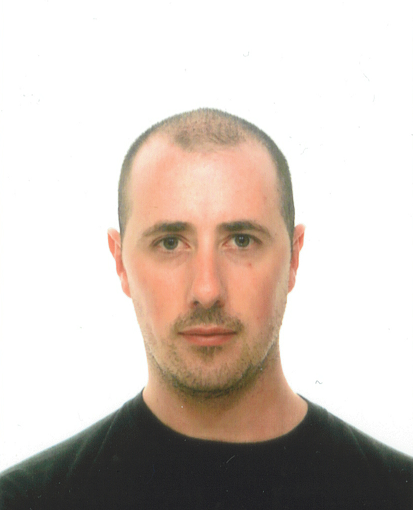
\includegraphics[width=.25\textwidth]{input/face.png}\vspace{.3cm}\\
Iriarte, 14-16, 1, 2 \textbar{} 08191 \textbar{} Rubí (Barcelona) \textbar{} Spain\\
+34 622895156 \textbar{} salcantaraphd@gmail.com  \vspace{0.2cm}\\
} % put your contact information here

\date{} % Leave blank to remove the date

\begin{document}
\maketitle
\vspace{-1cm}

%\section{Personal Details}
%\begin{flushleft}
  %Gender: Male \\
%  Date of birth: 18th of May, 1981 \\
%  Place of birth: Barcelona, Spain \\
  %Present citizenship: Spanish \\
%\end{flushleft}


\section{Education}

\begin{CV}

\item[10/2008--10/2011] PhD in Industrial Informatics\\
Dept. of Telecommunications and Systems Engineering \\
Universitat Autònoma de Barcelona (UAB, \url{www.uab.es}) \\
\\
Doctoral Thesis: \emph{Analytical design of feedback compensators based on robustness/performance and servo/regulator trade-offs: \small{utility in PID control applications}}\\

\item[09/2005--09/2008] MSc in \emph{Industrial Informatics}\\
Dept. of Telecommunications and Systems Engineering (UAB)\\

\item[09/2006--01/2012] BSc in Mathematics (3-year degree)\\
UAB, Faculty of Sciencies (\url{http://www.uab.cat/matematiques/})\\

\item[09/1999--02/2005] BSc in Computer Science/Engineering (5-year degree)\\
UAB, School of Engineering\\ (\url{http://www.uab.es/escola-enginyeria/})
\\Most relevant courses: databases, signal processing,
cryptography, artificial intelligence, robotics, compilers,
automatic control, software engineering, networking, computer vision...
\vspace{0.2cm}
\\Diploma Thesis: \emph{Fast Discrete Wavelet Transform}
%Carried out at the
%Communications and Information Engineering Dept. (\url{http://deic.uab.cat/})\\
%Directed by: Joan Serra Sagristà (Email: \url{joan.serra@deic.uab.cat}).
\\

\item[09/1995--06/1999] Secondary school (BUP and COU).\\ 
VIARÓ (private school, \url{www.viaro.es}), 08174, Sant Cugat del Vallès (Barcelona).\\
\\
\hspace{0.2cm} \emph{Honours and Awards}: \hspace{0.2cm}

\begin{CV}
\item[COU] Extraordinary Award (got my first year at university for free)\\
\end{CV}
\end{CV}

\pagebreak

\section{Working Experience}
\begin{CV}
\item[09/2012--09/2014] Postdoctoral fellow\\
Marie Curie researcher within the european IAPP project \emph{Next Air Biotreat}, grant number 284949 \\ 
(\url{http://www.nextairbiotreat.eu/})\\
Pure Air Solutions (\url{www.pureairsolutions.nl})\\
Zwolle, The Netherlands
\vspace{0.4cm}\\TASKS:\vspace{0.2cm}
\begin{itemize}
\item Supervision of early stage researchers
\item Modelling and simulation using MATLAB 
%\item Writing small programs for the design of chemical scrubbers and Gas-Liquid-Solid (GLS) separators in anaerobic reactors
\item PLCs/SCADA programming for the control of industrial biotrickling filters (PLC used: TBOX MS32 from CSE Semaphore)
\item Design and implementation of a web-based monitoring platform for the company's PLCs data. Technologies used:
\begin{itemize}
\item VB.NET, MODBUS/TCP 
\item HTML, CSS, Javascript and PHP (Yii framework)
\item MySQL database 
\item Git version control system
\end{itemize}
\end{itemize}


\item[10/2011--09/2012] Postdoctoral fellow\\
Postdoctoral researcher at UAB (research and teaching tasks) \\
Dept. of Telecommunications and Systems Engineering
\item[09/2007--09/2011] Predoctoral Scholar\\
PhD student and teaching assistant at UAB\\
Dept. of Telecommunications and Systems Engineering
\item[09/2005--09/2007] Assistant Professor at UAB\\
Dept. of Telecommunications and Systems Engineering
\vspace{0.2cm}
\noindent \\Teaching within the Computer Engineering degree:
\begin{itemize}
\item Signals and Systems (3rd year subject, only labs)
\item Signal processing (3rd year subject, only labs)
\item Automatic Control (4th year subject, only labs)
\item Director of around 10 final degree projects
\end{itemize}
Teaching within the (Technical) Telecommunication Engineering degree:
\begin{itemize}
\item Control Systems (3rd year subject, only labs)
\end{itemize}

\item[07/2004--09/2005] Junior programmer at the software department
of Intelogistica (\url{www.intelogistica.com}), later Coordina (\url{www.coordina.com}), and finally acquired by TomTom (\url{http://www.tomtom.com/})
\vspace{0.4cm}\\TASKS:\vspace{0.15cm}
\begin{itemize}
\item Symbian smartphones programming in C++. Design and implementation of GPS-based applications
\item Brief exposure to some java frameworks (Hibernate, Spring)
\end{itemize}


\item[06/2003--07/2004] Apache+Mysql+PHP Junior web programmer. Some
projects in which I was involved can still be found at:\\
\vspace{-0.4cm}
\begin{center}\url{http://www.track.es/modulos/portfolioweb.php}\end{center}

\end{CV}


\section{Further Education / Training}

\begin{CV}

\item[03/2014] OPC Connectivity\\
Hands-on training workshop by MatrikonOPC (OPCSI certified), days 25--27 of March.
Barcelona, Spain
\vspace{0.2cm}\\COVERED TOPICS:\vspace{0.15cm}
\begin{itemize}
\item OPC Training Level 1\&2 -- OPC Integration \& Diagnostics (includes the OPC UA specification)
\item OPC Training Level 3 -- Implementing OPC Projects \& Advanced Architectures 
\end{itemize}
More info can be found in \url{http://www.matrikonopc.com/training/}

\item[9/2013] Online course by \url{mejorando.la}\\
Original title (in Spanish):\\ \emph{Curso profesional de frontend}
\vspace{0.2cm}\\COVERED TOPICS:\vspace{0.15cm}
\begin{itemize}
\item HTML5, CSS3, Javascript, Responsive Design, Backbone.js, CSS precompilers (Stylus), VCSs (Git)
\end{itemize}
More info can be found in \url{https://mejorando.la/cursos/}

\item[9/2013] Android programming\\
Online course by \url{mejorando.la}\\
Original title (in Spanish):\\ \emph{Curso de programación en Android}\\
More info can be found in \url{https://mejorando.la/cursos/}

\item[9/2013] BackendPro\\
Online course by \url{mejorando.la}\\
Original title (in Spanish):\\ \emph{Curso profesional de backend}
\vspace{0.2cm}\\COVERED TOPICS:\vspace{0.15cm}
\begin{itemize}
\item Databases (MySQL, MongoDB),Python/Django, Node.js
\end{itemize}
More info can be found in \url{https://mejorando.la/cursos/}

\item[10/2010--12/2010] Visiting researcher\\
Research period in Trondheim (Norway)\\
Norwegian University of Science and Technology (NTNU)\\
Deparment of Chemical Engineering, Process Control Group\\
Supervised by Prof. Sigurd Skogestad

\item[09/2009--12/2009] Visiting researcher\\
Research period in Shanghai (P.R. China)\\
Shanghai Jiao Tong University (SJTU)\\
Deparment of Automation\\
Financial support received from the AGAUR research funds BE-DGR 2009 (\url{www.gencat.cat/agaur/})\\
Supervised by Prof. Weidong Zhang

\end{CV}

\section{Language Knowledge}
\begin{CV}

%\item[Catalan] Native
\item[English]
\textbf{12/2007} Advanced Certificate in English (CAE) \\ University of
Cambridge.
\item[Spanish/Catalan] Mother tongues
(bilingual)
\end{CV}


\section{Interests and activities}
\begin{itemize}
\item Process control and automation (OPC, SCADA, PLCs, PID control...)
\item Web/mobile apps development
\item Databases, Big Data, data science, machine learning...
\item Home and private tutor for primary and secondary education levels
%Private English teacher at Chaplin's School (\url{http://www.chaplins.org/}) for Junior Pre-Intermediate level (only during the course 2008-2009). Contact person: Thomas Frahm (Email: \url{tfrahm@chaplins.org})
\item Others: fitness/bodybuilding, listening to music, getting relaxed...
\end{itemize}


\pagebreak

\section{References}

\noindent These persons are familiar with my qualifications/character:\\


\textbf{Prof. Weidong Zhang} \\
Shanghai Jiao Tong University (SJTU), Department of Automation\\
200240 Shanghai (P.R. China)\\
Phone: +86 21 34204021, Email: \url{wdzhang@sjtu.edu.cn}\\
Homepage: \url{http://automation.sjtu.edu.cn/wdzhang/}\\


\textbf{Prof. Sigurd Skogestad} \\
Norwegian University of Science and Technology (NTNU) \\
Department of Chemical Engineering, N-7491 Trondheim (Norway)\\
Phone: +47 735 94154, Email: \url{skoge@ntnu.no} \\
Homepage: \url{http://www.nt.ntnu.no/users/skoge/}\\


\textbf{Prof. Ramon Vilanova} \\
Head of the research group:\\
\emph{Automation and Advanced Control Systems} (\url{http://tes.uab.es/TC})\\
UAB, Department of Telecommunications and Systems Engineering\\
08193 Bellaterra (Cerdanyola), Barcelona (Spain) \\
Phone: +34 93 581 2197, Email: \url{ramon.vilanova@uab.es} \\


\textbf{MSc Cristian Martí} \\
General Manager Software Engineering in TomTom Business Solutions, before:
CEO at Coordina (\url{www.coordina.com}), now a TomTom company\\
Linkedin: \url{http://www.linkedin.com/in/cristianmarti}\\
Email: \url{c.marti@coordina.com}\\

\textbf{MSc Albert Waalkens} \\
CEO at Pure Air Solutions (\url{www.pureairsolutions.nl})\\
Linkedin: \url{http://nl.linkedin.com/pub/albert-waalkens/0/501/560}\\
Email:  \url{a.waalkens@pureairsolutions.nl} \\


\section{Public profiles}
\begin{flushleft}
  \url{https://www.linkedin.com/in/salvalcantara/}
\end{flushleft}
\begin{flushleft}
  \url{https://scholar.google.com/citations?user=iAEKXqQAAAAJ}
\end{flushleft}
\begin{flushright}
\vspace{2\baselineskip} \noindent Barcelona, Spain, \today
\end{flushright}


\section{Dummy section}\label{dummy-section}

\begin{description}
\item[09/2009--12/2009]
Visiting researcher\newline
 Research period in Shanghai (P.R. China)\newline
 Shanghai Jiao Tong University (SJTU)\newline
 Deparment of Automation\newline
 Financial support received from the
\href{http://www.gencat.cat/agaur/}{AGAUR} research funds BE-DGR
2009\newline
 Supervised by Prof.~Weidong Zhang\newline
\item[09/2009--12/2009]
Visiting researcher\newline

\begin{verbatim}
Research period in Shanghai (P.R. China)
\end{verbatim}

\begin{verbatim}
Shanghai Jiao Tong University (SJTU)
\end{verbatim}

\begin{verbatim}
Deparment of Automation
\end{verbatim}

\begin{verbatim}
Financial support received from the [AGAUR](http://www.gencat.cat/agaur/) research funds BE-DGR 2009
\end{verbatim}

\begin{verbatim}
Supervised by Prof. Weidong Zhang
\end{verbatim}
\end{description}

\section{References}\label{references}

These persons are familiar with my professional qualifications and my
character:

\textbf{Prof.~Weidong Zhang}\\
Shanghai Jiao Tong University, Department of Automation\\
Phone: +86 21 34204021, Email:
\href{mailto:wdzhang@sjtu.edu.cn}{\nolinkurl{wdzhang@sjtu.edu.cn}}\\
Homepage: \url{http://automation.sjtu.edu.cn/wdzhang/}

\textbf{Prof.~Sigurd Skogestad}\\
Norwegian University of Science and Technology\\
Phone: +47 735 94154, Email:
\href{mailto:skoge@ntnu.no}{\nolinkurl{skoge@ntnu.no}}\\
Homepage: \url{http://www.nt.ntnu.no/users/skoge/}

\textbf{Prof.~Ramon Vilanova}\\
UAB, Department of Telecommunications and Systems Engineering\\
08193 Bellaterra (Cerdanyola), Barcelona, Spain\\
Phone: +34 93 581 2197, Email:
\href{mailto:ramon.vilanova@uab.es}{\nolinkurl{ramon.vilanova@uab.es}}

\textbf{MSc Cristian Martí}\\
Founder at \href{http://methinks.es/}{Methinks}\\
Former CEO at \href{www.coordina.com}{Coordina}, now a TomTom company\\
Linkedin: \url{http://www.linkedin.com/in/cristianmarti}

\textbf{MSc Albert Waalkens}\\
CEO at \href{www.pureairsolutions.nl}{Pure Air Solutions}\\
Linkedin: \url{http://nl.linkedin.com/pub/albert-waalkens/0/501/560}\\
Email:
\href{mailto:a.waalkens@pureairsolutions.nl}{\nolinkurl{a.waalkens@pureairsolutions.nl}}

\end{document}
